\documentclass[12pt]{article}
\usepackage[utf8]{inputenc}
\usepackage{longtable}
\usepackage{multirow}
\usepackage{graphicx}
\graphicspath{ {./author/} }


\renewcommand{\baselinestretch}{1.5}

\title{Emily Post(1873-1954)}
\author{Luis Diego Jiménez Delgado}
\date{Agosto 12 del 2019}

\begin{document}

\maketitle

\begin{center}
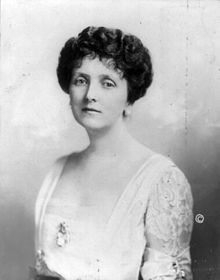
\includegraphics{po}
\end{center}
De pequeña, fue educada en su hogar y en escuelas privadas. Conoció a su esposo, Edwin, en un baile durante su período de "presentación en sociedad". (Hace años, las jovencitas eran presentadas en sociedad en una serie de fiestas y bailes). Después de que sus dos hijos se fueron a la universidad, ella comenzó a escribir.
Emily Post era una escritora única, que trabajaba con un propósito particular. Su tema principal era instruir a las personas sobre los buenos modales, o etiqueta. �Qué es la etiqueta? Son reglas de conducta que indican la manera apropiada en que las personas deben comportarse en diversas situaciones. Puede incluir información sobre buenos modales y también habilidades sociales tales como vestimenta adecuada y acciones apropiadas en diversas situaciones.
Comenzó a escribir para ganarse la vida y publicó varios artículos e historias sobre temas tales como decoración de interiores e historias de ficción. Uno de sus editores le pidió que escribiera sobre etiqueta y así lo hizo, publicando en 1922 La Etiqueta en la Sociedad, los Negocios, la Política y el Hogar
\end{document}